

\chapter{Verificarea formală a problemei}

\section{Schema verificării}
    \vspace{1cm}
\setcounter{figure}{0}
    \begin{figure}[h]
        \centering
          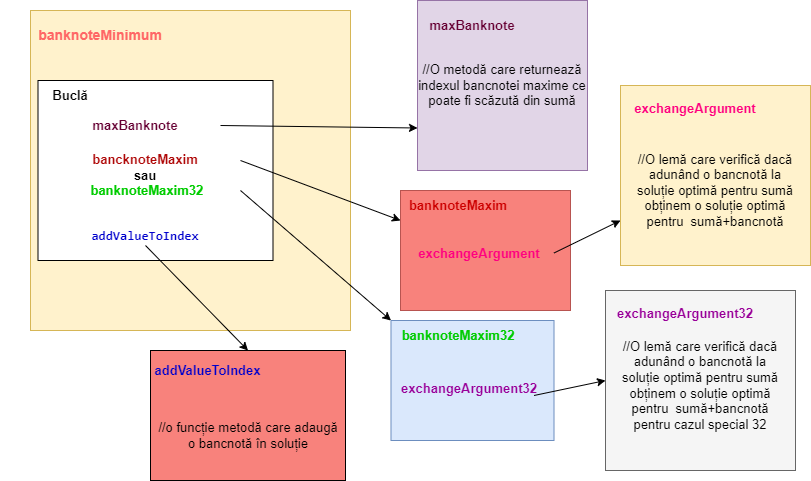
\includegraphics[width=1.0\textwidth]{verification_schema}
      \end{figure}
Figura 1: O schemă explicativă a apelurilor de funcții și leme în cadrul verificării.
    

\section{Demonstrarea optimalității}

    Pentru a demonstra că o soluție este optimă, încercăm să găsim o soluție cu cost mai mic, dacă nu reușim, atunci 
    știm că soluția găsită este optimă.\cite{kozen1993optimal}
  
  \subsection{Metoda banknoteMinimum}
    Metoda banknoteMinimum este metoda principală folosită pentru a returna soluția optimă pentru o sumă dată ca 
    input.\par
    Această metodă are ca precondiții faptul că suma este pozitivă, iar ca postcondiții avem cele 3 predicate menționate 
    anterior care asigură optimalitatea unei soluții.\par
    Metoda folosește o buclă, în care, la fiecare iterație, se adaugă o bancnotă în soluție.\par
    Invarianții prezenți în while au rolul de a menține proprietatea de optimalitate 
    pe parcursul construirii soluției, astfel că la orice pas soluția este optimă pentru $suma-rest$ de la momentul respectiv.\par
    În primă fază calculează bancnota cea mai mare ce poate fi dată ca rest, cu ajutorul funcției maxBanknote și funcției 
    power.\par
    Ulterior, folosește lema banknoteMaxim sau banknoteMaxim32, în funcție de bancnota aleasă, pentru a demonstra 
    că dacă adaugăm bancnota aleasă la soluția calculată până în prezent, noua soluție pentru $sum-rest$ adunată cu o 
    soluție optimă pentru $rest - bancnota$ produce o soluție optimă pentru sumă .\par
    
    \begin{lstlisting}
    method banknoteMinimum(sum: int) returns(solution: seq <int> )
        requires sum >= 0
        ensures isValidSolution(solution)
        ensures isSolution(solution, sum)
        ensures isOptimalSolution(solution, sum) 
    {
        var rest:= sum;
        solution:= [0, 0, 0, 0, 0, 0];
        var index:= 0;
        assert isOptimalSolution(solution, sum - rest);
        while (0 < rest)
            invariant 0 <= rest <= sum
            invariant isValidSolution(solution)
            invariant addOptimRestEqualsOptimSum(rest, sum, solution)
            decreases rest 
        {
            index:= maxBanknote(rest);
            var banknote:= power(2, index);
            if (index != 5) 
            {
                banknoteMaxim(rest, sum, solution, index);
            } 
            else 
            {
                banknoteMaxim32(rest, sum, solution);
            }
            solution:= addValueToIndex(solution,1,index);
            rest:= rest - banknote;
        }
    }
    \end{lstlisting}

    \subsection{Metoda maxBanknote}
    Metoda maxBanknote este folosită pentru a returna un index cu proprietatea: \par
     $bancnota_{index} <= rest < bancnota_{index + 1}$  .\par
     Avem postcondițiile următoare: indexul să se afle în range-ul secvenței, bancnota corespunzătoare indexului să fie mai mică decât suma,
     și un index nu poate fi mai mare decât a fost calculat fără depăși suma.
     Aceste postcondiții au fost necesare pentru a demonstra faptul că indexul returnat este întradevăr corespunzător celei
     mai mari bancnote care poate fi dată rest pentru sum.
    \begin{lstlisting}
      method maxBanknote(sum: int) returns(index: int)
        requires sum > 0
        ensures 0 <= index <= 5
        ensures 0 <= power(2, index) <= sum
        ensures(index != 5 && power(2, index + 1) > sum) || index == 5 
      {
        index:= 5;
        if (power(2, index) > sum) 
        {
          assert power(2, index + 1) > sum;
          while (power(2, index) > sum && index > 0)
            invariant power(2, index + 1) > sum 
            {
              index:= index - 1;
              assert power(2, index + 1) > sum;
            }
        } 
          else 
        {
          assert index == 5;
        }
      }
    \end{lstlisting}


    \subsection{Lema banknoteMaxim sau banknoteMaxim32}
    Lema banknoteMaxim,  respectiv banknoteMaxim32, este folosită pentru a demonstra faptul că dacă adăugam o bancnotă în soluția pe care o 
    construim, în continuare suma acestei soluții cu soluția optimă pentru $ rest - bancnota$ va produce soluția 
    optimă pentru suma întreagă.\par
    Pentru a demonstra acest lucru avem nevoie să știm că dacă în soluția curentă, optimă pentru $ rest - bancnota$  
    adaugăm bancnota aceasta devine optimă pentru $rest$. Acest lucru este demonstrat cu ajutorul lemei exchangeArgument, respectiv exchangeArgument32.
    Cele doua leme sunt similare așa că voi da exemplu de cod doar pentru una dintre ele.\par
    Aceste lemme au nevoie ca indexul să se afle în range și să fie ales conform metodei maxBanknote, soluția calculată până 
    în prezent să fie validă și să respecte predicatul addOptimRestEqualsOptimSum, așadar acestea sunt precondițiile.
    Această metodă asigură că predicatul addOptimRestEqualsOptimSum este valid și pentru $rest $ dacă scădem bancnota aleasă din rest, 
    de aceea este postcondiție.
    \begin{lstlisting}
    lemma banknoteMaxim(rest: int, sum: int, finalSolution: seq <int> , index: int)
        requires 0 <= index <= 4
        requires power(2, index) <= rest < power(2, index + 1)
        requires isValidSolution(finalSolution)
        requires addOptimRestEqualsOptimSum(rest, sum, finalSolution)
        ensures addOptimRestEqualsOptimSum(rest - power(2, index), sum, finalSolution[index:= finalSolution[index] + 1]) 
    {
        var banknote:= power(2, index);
        forall currentSolution | isValidSolution(currentSolution) && isOptimalSolution(currentSolution, rest - banknote)
            ensures isOptimalSolution(solutionsSum(solutionsSum(currentSolution, finalSolution), [0, 0, 0, 0, 0, 0][index:= 1]), sum) 
        {
            assert isSolution(currentSolution[index:= currentSolution[index] + 1], rest);
            exchangeArgument(rest, currentSolution, index);
        }
        assert forall currentSolution::isValidSolution(currentSolution) && isOptimalSolution(currentSolution, rest - banknote) ==> isOptimalSolution(solutionsSum(solutionsSum(currentSolution, finalSolution), [0, 0, 0, 0, 0, 0][index:= 1]), sum);
    }
    \end{lstlisting}

    \subsection{Lema exchangeArgument sau exchangeArgument32}
    Lema exchangeArgument, respectiv exchangeArgument32, presupune că nu este optimă soluția dacă adaugăm bancnota aleasă și ajunge la o contradicție.
    Știm că soluția e optimă pentru $rest - bancnota$, dar nu pentru rest, dacă adaugăm bancnota.\par
    Consideră că există o altă soluție optimă pentru rest.\par
    Următoarea verificare este specifică cazurilor $1,2,4,8,16$.\par
    $\bullet $ Verificăm în presupusa soluție pentru rest că nu avem bancnota în soluție deja, altfel dacă din acea presupusă 
     solutie am scădea bancnota, atunci am avea un cost mai mic decât costul soluției noastre care e optimă pentru 
     $rest - bancnota$ din precondiție, deci avem o contradicție.
    Ulterior, verificăm demonstrăm că invariantul explicat în subsecțiunea 2.3.1 se menține pe parcursul unei bucle.\par
    Nu există două bancnote de aceeași valoare în soluție, mai mici de 32.\par
    În acest mod știm că soluția presupusă nu poate fi optimă, deoarece, dacă respectă proprietatea
    suma produsă de aceasta nu poate fi egală cu rest. \par
    Deoarece :\par
    $\bullet \sum_{k=0}^{index-1} 2^{k} = 2^{index}-1 $\par
    $\bullet rest > = 2^{index} $ \par
    Deci presupusa soluție pentru rest nu poate fi egală decât cu cel mult $rest- 1$, astfel nu poate fi soluție optimă și se ajunge la o contradicție. 
    Precondițiile și postcondițiile necesare pentru acestor lemme sunt aceleași ca în lemma banknoteMaxim, respectiv banknoteMaxim32.\par
    Lemma exchangeArgument este o lemă tipică algoritmilor greedy care se bazează pe ideea că modificând progresiv 
    dintr-o soluție produsă de orice alt algoritm într-o soluție produsă de algoritmul greedy, dacă folosim un mod 
    care să nu înrăutățească calitatea soluției, atunci costul soluției produse este cel puțin la fel de mic ca 
    cea a oricărei alte soluții, acesta fiind argumentul de schimb.\par
    \begin{lstlisting}
lemma exchangeArgument(rest: int, currentSolution: seq <int> , index: int)
    requires 0 <= index <= 4
    requires power(2, index) <= rest < power(2, index + 1)
    requires isValidSolution(currentSolution)
    requires isOptimalSolution(currentSolution, rest - power(2, index))
    ensures isOptimalSolution(currentSolution[index:= currentSolution[index] + 1], rest) 
{
    var banknote:= power(2, index);
    var solution:= currentSolution[index:= currentSolution[index] + 1];
    assert isValidSolution(solution);
    assert isSolution(solution, rest);
    var i:= index;
    if (!isOptimalSolution(solution, rest)) 
    {
    var optimalSolution:| isValidSolution(optimalSolution) && isSolution(optimalSolution, rest) &&
        isOptimalSolution(optimalSolution, rest) && cost(optimalSolution) < cost(solution);
    if (optimalSolution[index] -1 >= 0) 
    {
        var betterSolution:= addValueToIndex(optimalSolution,-1,index);
        assert isSolution(betterSolution, rest - banknote);
        assert cost(betterSolution) == cost(optimalSolution) - 1;
        assert cost(optimalSolution) - 1 < cost(currentSolution);
        assert false;
    } 
    else 
    {
        while (0 < i)
        invariant 0 <= i <= index
        invariant forall x::index >= x >= i ==> optimalSolution[x] <= 1 
        {
        i:= i - 1;
        assert isOptimalSolution(optimalSolution, rest);
        if (optimalSolution[i] > 1) 
        {
            var optimalSolution' := optimalSolution[i:=optimalSolution[i]-2];
            optimalSolution' := optimalSolution' [i + 1:= optimalSolution'[i+1]+1];
            assert isSolution(optimalSolution', rest);
            assert cost(optimalSolution') == cost(optimalSolution) - 1;
            assert cost(optimalSolution') < cost(optimalSolution);
            assert false;
        }
        }
        assert solutionElementsSum(optimalSolution) <= banknote - 1;
        assert rest >= banknote; 
        assert solutionElementsSum(optimalSolution) <= rest - 1; 
        assert isOptimalSolution(optimalSolution, rest); 
        assert false;
        }
    }
}
    \end{lstlisting}
        
    

\subsection{Funcția addValueToIndex}
Funcția addValueToIndex este folosită pentru a adăuga unui element din soluție o valoare, folosindu-ne de index-ul acestuia.\par
Este utilă pentru construirea soluțiilor.\par
Aceasta are drept precondiții pentru modificarea corectă a sumei faptul că index-ul trebuie să fie în range, soluția să fie validă și
faptul că valoarea adaugată plus valoarea inițială a elementului din secvență nu reprezintă un număr negativ.\par
Postcondițiile acestei funcții ne asigură faptul că avem o soluție validă în urma adaugării și faptul că valoarea sumei pe care 
o reprezintă soluția a crescut cu valoarea la care ne așteptam.\par
\begin{lstlisting}
function method addValueToIndex(solution: seq<int>, value: int, index: int): seq<int>
  requires 0 <= index <= 5
  requires isValidSolution(solution)
  requires solution[index] + value >= 0
  ensures isValidSolution(solution)
  ensures solutionElementsSum(solution) + value*power(2, index) == solutionElementsSum(solution[index:=solution[index]+value])
{
  solution[index:= solution[index] + value]
}
\end{lstlisting}
